\section{Termine}

\begin{figure}[b]
  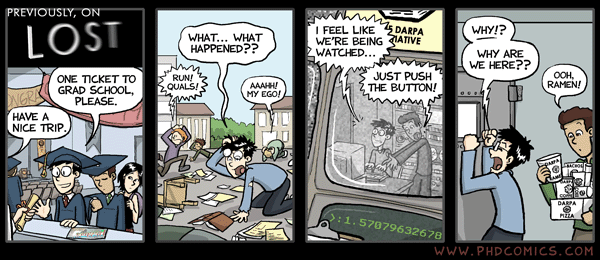
\includegraphics[width=\textwidth ]{bilder/comics/phd092706s.png}
\end{figure}

Gerade in der Anfangszeit des Studiums gibt es eine Menge zu tun. Damit ihr
nicht das Wichtigste verpasst, haben wir die ersten Termine kompakt f"ur
euch zusammengefasst. Die meisten davon bieten die Gelegenheit Fragen zu
stellen und nebenbei gleich ein paar nette Kommilitonen kennen zu lernen.

Das K"urzel nach Datum und Zeit gibt den Raum bzw. Ort an. F"ur alle R"aume die nicht
im IZ (steht f"ur Informatikzentrum) liegen, schaut am besten auf den
Raumplan. Bei den R"aumen im IZ ist die erste Zahl das Stockwerk, f"ur
den Rest m"usst ihr dann auf den Plan im Stockwerk schauen (Kleine Falle:
zwischen EG und 1. OG liegt das Galeriegescho"s - Raum 149/150 liegt also
effektiv in der zweiten Etage).\par
\newpage
\begin{description}
  \item[Do, 24.09. ~~ 17 Uhr] \hfill \nroom{IZ 161}\\
    Einf"uhrungsveranstaltung der Fachgruppe
  \item[Mo, 28.09. -- Fr, 09.10.]
    Vorkurs Mathematik
  \item[Di, 20.10. ~~ 10 Uhr] \hfill \nroom{Plaza im IZ} \\
    Erstsemesterfr"uhst"uck der Informatik
  \item[Di, 20.10. ~~ 11:30 Uhr] \hfill \nroom{IZ 161} \\
    Einf"uhrungsveranstaltung der Fachgruppe
  \item[Di, 20.10. ~~ 13 Uhr] \hfill \nroom{IZ 161} \\
    Campusf"uhrung in Tutorengruppen
  \item[Mo, 19.10. ~~ 15 Uhr] \hfill \nroom{SN 19.1}\\
    Erste Vorlesung: "`Programmieren I"'
  \item[Mi, 21.10.] \hfill \nroom{ganzer Campus}\\
    Studium Generale: Interessante Vorlesungen aus allen Fachrichtungen
  \item[Di, 03.11.] \hfill \nroom{IZ 150}\\
    Spieleabend der Fachgruppe
\end{description}


% - Erig-Party im AM
% - Gl"uhweinabend im Informatikzentrum (IZ)
